% Companion document for safod_solid_earth_tide_2026-06-17.png
% Compile with pdflatex, twice if cross-references are added later.
\documentclass[11pt]{article}

\usepackage[margin=1in]{geometry}
\usepackage[T1]{fontenc}
\usepackage{lmodern}
\usepackage{amsmath,amssymb}
\usepackage{booktabs}
\usepackage{graphicx}
\usepackage{xcolor}
\usepackage[hidelinks]{hyperref}

\setlength{\parskip}{0.45em}
\setlength{\parindent}{0pt}
\newcommand{\eps}{\varepsilon}
\newcommand{\dvv}{\delta v/v}
\newcommand{\Rearth}{R_{\oplus}}

\title{\textbf{Reading the SAFOD Solid--Earth Tide Model}}
\author{Companion to the June 17, 2026 SAFOD active-source DAS experiment}
\date{\today}

\begin{document}
\maketitle

\begin{abstract}
This short note derives the first-pass model used to make
\texttt{safod\_solid\_earth\_tide\_2026-06-17.png}.  The calculation predicts
the astronomical solid-Earth forcing at SAFOD from the Sun and Moon, then
converts that forcing into a scalar areal-strain proxy with degree-2 Love
numbers.  It does \emph{not} yet predict the seismic velocity change measured
by DAS.  That conversion requires an unknown rock-and-observable sensitivity.
\end{abstract}

\section{What quantity is plotted?}

The upper panel plots the modeled scalar tidal strain
\begin{equation}
  \eps_{\mathrm{tide}}(t),
\end{equation}
not the measured seismic velocity change.  Strain is dimensionless:
\begin{equation}
  \eps = \frac{\Delta L}{L}.
\end{equation}
For example, $\eps=4\times10^{-8}$ means that a one-metre length would change
by $4\times10^{-8}$ m in this idealized scalar description.

The figure uses nano-strain, abbreviated n$\eps$ or n$\varepsilon$:
\begin{equation}
  1\,\mathrm{n}\eps = 10^{-9},
  \qquad
  40\,\mathrm{n}\eps = 40\times10^{-9}=4\times10^{-8}.
\end{equation}
Thus the vertical axis is labeled
``areal strain $\times 10^9$ (n$\eps$)''.  The plotted number is the
dimensionless strain multiplied by $10^9$ for readability.  It is not a unit
of metres, metres per second, or fractional velocity.

The lower panel is dimensionless in a different sense: it is a normalized
shape.  Define
\begin{equation}
  \tau(t) =
  \frac{\eps_{\mathrm{tide}}(t)-\overline{\eps_{\mathrm{tide}}}}
       {\max_t\left|\eps_{\mathrm{tide}}(t)-\overline{\eps_{\mathrm{tide}}}\right|}.
\end{equation}
Then $\tau$ has no physical amplitude and ranges approximately from $-1$ to
$+1$.  It is the known time shape used as a matched-filter template.

\section{The physical coupling to apparent velocity}

The measurement from repeated active-source waveforms is an apparent
fractional velocity change, which we denote by $y(t)$:
\begin{equation}
  y(t) = \left(\frac{\delta v}{v}\right)_{\!\mathrm{app}}(t).
\end{equation}
For a fixed travel path, a small perturbation obeys
\begin{equation}
  \frac{\delta t}{t} = -\frac{\delta v}{v}.
\end{equation}
The simplest tide-response model is
\begin{equation}
  y(t) = A\,\tau(t) + c_0+c_1t+c_2t^2+\eta(t),
  \label{eq:fit}
\end{equation}
where $A$ has units of fractional velocity change, the $c$ terms absorb slow
experimental drift, and $\eta$ is noise.  The coefficient $A$ is not equal to
the strain.  It represents the observed velocity response after the unknown
rock physics, fractures, fluids, stress state, and measurement coupling have
acted on the forcing.

Equivalently, before normalizing the template one can write
\begin{equation}
  \left(\frac{\delta v}{v}\right)_{\!\mathrm{tide}}
  = S\,\eps_{\mathrm{tide}},
  \label{eq:sensitivity}
\end{equation}
where $S$ is a dimensionless strain sensitivity.  Equation~\eqref{eq:sensitivity}
is a constitutive or empirical coupling assumption; it does not follow from
the astronomical tide calculation alone.

\section{Step 1: site and time}

The model uses
\begin{align}
  \phi &= 35.9746^\circ, &
  \lambda &= -120.5516^\circ,
\end{align}
with east-positive longitude.  The time series covers
2026-06-16 23:48 through 2026-06-17 23:44 UTC at one-minute spacing, giving
1437 samples.  For each time, the code calculates the Julian Date and
\begin{equation}
  d = \mathrm{JD}-2451545.0,
\end{equation}
the number of days since J2000.0.

The UTC convention matters.  Shifting the time series by several hours shifts
the local hour angle and therefore shifts the phase of the predicted tide.

\section{Step 2: Sun and Moon geometry}

For each body $b$, the model needs right ascension $\alpha_b$, declination
$\delta_b$, and geocentric distance $D_b$.  The short-period solar formulas
use a mean longitude $L_\odot$ and mean anomaly $g_\odot$:
\begin{align}
  \lambda_\odot &= L_\odot
    +1.915^\circ\sin g_\odot+0.020^\circ\sin(2g_\odot),\\
  R_\odot &= 1.00014-0.01671\cos g_\odot
    -0.00014\cos(2g_\odot).
\end{align}
The ecliptic longitude is rotated into equatorial coordinates using the
obliquity $\epsilon_{\mathrm{ecl}}$:
\begin{align}
  \alpha &= \operatorname{atan2}\!\left(\cos\epsilon_{\mathrm{ecl}}\sin\lambda,
                    \cos\lambda\right),\\
  \delta &= \arcsin\!\left(\sin\epsilon_{\mathrm{ecl}}\sin\lambda\right).
\end{align}

The Moon is computed from a truncated Keplerian orbit with semimajor axis
$a=60.2666\Rearth$, eccentricity $e=0.054900$, inclination
$i=5.1454^\circ$, and time-dependent orbital angles.  The orbital-plane
coordinates are rotated through the ascending node, inclination, and
argument of perigee, then into the equatorial frame.  This is appropriate for
understanding the signal shape over one day, but not for precision gravimetry.

At the SAFOD site, the local sidereal time is
\begin{equation}
  \mathrm{LST} =
  \left(280.46061837+360.98564736629d+\lambda\right)\bmod 360^\circ.
\end{equation}
The hour angle is $H_b=\mathrm{LST}-\alpha_b$.  The body-to-site zenith angle
$\theta_b$ follows from
\begin{equation}
  \cos\theta_b =
  \sin\phi\sin\delta_b
  +\cos\phi\cos\delta_b\cos H_b.
\end{equation}

\section{Step 3: degree-2 tidal potential}

The dominant body-tide term is the degree-2 part of the tide-generating
potential.  For body $b$,
\begin{equation}
  W_b(t) =
  \frac{G M_b}{D_b(t)^3}\,\Rearth^2\,
  P_2\!\left(\cos\theta_b(t)\right),
  \label{eq:potential}
\end{equation}
where
\begin{equation}
  P_2(x)=\frac{3x^2-1}{2}
\end{equation}
is the second Legendre polynomial.  The total potential is
\begin{equation}
  W(t)=W_{\mathrm{Moon}}(t)+W_{\mathrm{Sun}}(t).
\end{equation}

The units are important:
\begin{equation}
  [G M/D^3] = \mathrm{s}^{-2},
  \qquad [\Rearth^2]=\mathrm{m}^2,
  \qquad [W]=\mathrm{m}^2\,\mathrm{s}^{-2}.
\end{equation}
The $D^{-3}$ factor is the signature of a tide: the relevant forcing is the
spatial variation of gravity across Earth, not the uniform gravitational
acceleration of the whole Earth--Moon or Earth--Sun system.

\section{Step 4: potential to scalar strain}

The quantity
\begin{equation}
  \frac{W}{g\Rearth}
\end{equation}
is dimensionless because $g\Rearth$ has units of
$(\mathrm{m}\,\mathrm{s}^{-2})\mathrm{m}=\mathrm{m}^2\mathrm{s}^{-2}$.
The model then applies the degree-2 Love-number factor:
\begin{equation}
  \boxed{
  \eps_{\mathrm{tide}}(t)=
  \left(2h_2-6l_2\right)\frac{W(t)}{g\Rearth}}
  \label{eq:strain}
\end{equation}
with
\begin{center}
\begin{tabular}{@{}lll@{}}
\toprule
Symbol & Meaning & Value \\
\midrule
$\Rearth$ & Earth radius & $6.371\times10^6$ m \\
$g$ & surface gravity & $9.81$ m s$^{-2}$ \\
$h_2$ & radial Love number & $0.6032$ \\
$l_2$ & horizontal/Shida Love number & $0.0839$ \\
$G$ & gravitational constant & $6.674\times10^{-11}$ m$^3$ kg$^{-1}$ s$^{-2}$ \\
\bottomrule
\end{tabular}
\end{center}
For the selected values,
\begin{equation}
  2h_2-6l_2=0.7030.
\end{equation}

\section{What the generated plot says}

For this implementation, the total scalar strain over the experiment window
is approximately
\begin{align}
  \min(\eps_{\mathrm{tide}})&=-2.88\times10^{-8}=-28.8\,\mathrm{n}\eps,\\
  \max(\eps_{\mathrm{tide}})&=+4.98\times10^{-8}=+49.8\,\mathrm{n}\eps,\\
  \text{peak-to-peak}&=7.86\times10^{-8}=78.6\,\mathrm{n}\eps.
\end{align}
The unequal humps arise because the total signal is a sum of solar and lunar
terms, each containing diurnal and semidiurnal geometry.  The model predicts
the forcing shape and scale; it does not say that the measured $\dvv$ must be
$10^{-8}$.  A large or small measured $\dvv$ depends on $S$ in
Equation~\eqref{eq:sensitivity}.

\begin{figure}[ht]
  \centering
  \IfFileExists{safod_solid_earth_tide_2026-06-17.png}{%
    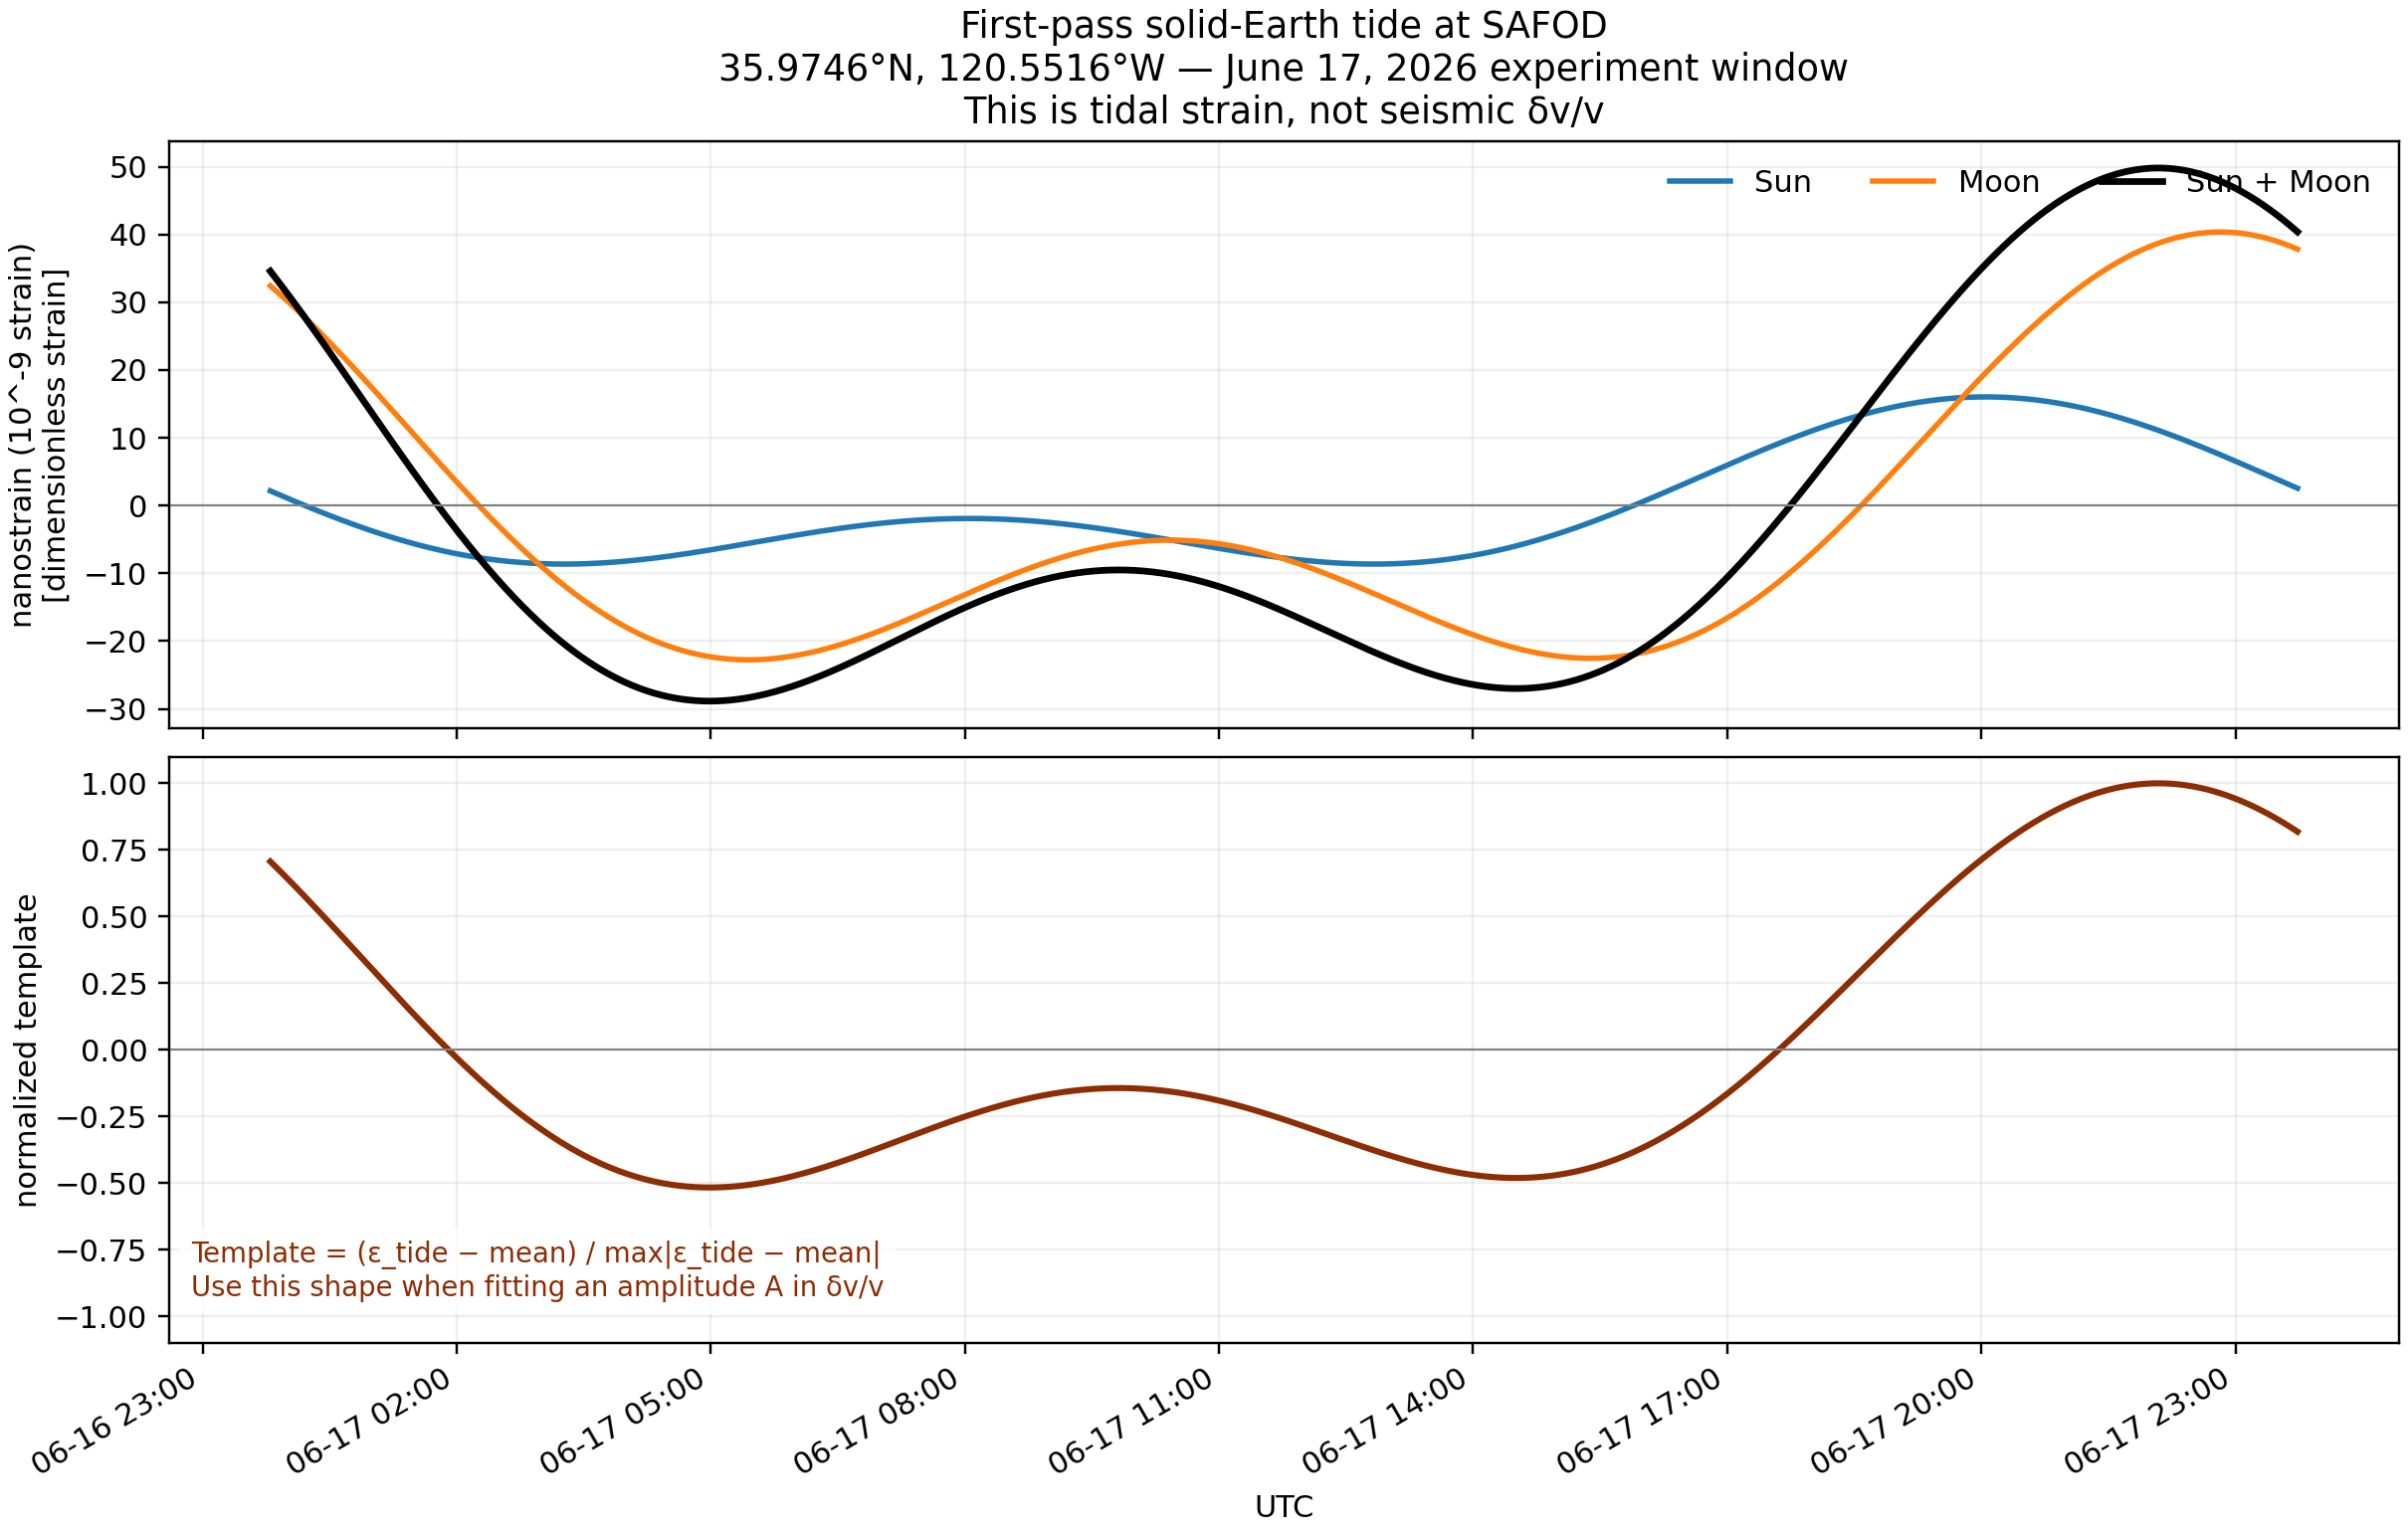
\includegraphics[width=0.98\textwidth]{safod_solid_earth_tide_2026-06-17.png}%
  }{\fbox{\parbox{0.9\textwidth}{Plot not found. Place
    \texttt{safod\_solid\_earth\_tide\_2026-06-17.png} next to this file.}}}
  \caption{Modeled scalar tidal strain and its normalized time shape.  The
  upper axis is dimensionless strain displayed in nano-strain; the lower axis
  is a unitless template for fitting apparent $\dvv$.}
\end{figure}

\section{Limitations to keep in view}

This calculation is a physically phased forcing model, not a full SAFOD
deformation solution.  A complete borehole DAS model would calculate the
strain tensor $\eps_{ij}$, include depth-dependent geometry and boundary
conditions, and project it onto the local fiber direction $n$:
\begin{equation}
  \eps_{\mathrm{fiber}}=n_i\eps_{ij}n_j.
\end{equation}
Ocean loading, atmospheric pressure, hydrology, local fault stress, and fluid
effects are also absent.  Finally, the Sun and Moon positions here use a
low-precision ephemeris.  The model is therefore suitable as a transparent
template and sensitivity calculation; precision tidal inference should use a
validated body-tide package and a tensor projection appropriate to the
downhole installation.

\begin{thebibliography}{9}
\bibitem{agnew}
D.~C. Agnew (2007), ``Earth tides,'' in \emph{Treatise on Geophysics},
2nd ed., Elsevier, doi:\href{https://doi.org/10.1016/B978-044452748-6.00056-0}{10.1016/B978-044452748-6.00056-0}.

\bibitem{farrell}
W.~E. Farrell (1972), ``Deformation of the Earth by surface loads,''
\emph{Reviews of Geophysics}, 10, 761--797,
doi:\href{https://doi.org/10.1029/RG010i003p00761}{10.1029/RG010i003p00761}.

\bibitem{metivier}
L.~M. M\'etivier and C.~P. Conrad (2008), ``Body tides of a convecting Earth,''
\emph{Journal of Geophysical Research}, 113, B11405,
doi:\href{https://doi.org/10.1029/2007JB005448}{10.1029/2007JB005448}.

\bibitem{takano}
K. Takano et al. (2014), ``Seismic velocity changes caused by the Earth tide,''
\emph{Geophysical Research Letters}, 41, 6131--6136,
doi:\href{https://doi.org/10.1002/2014GL060690}{10.1002/2014GL060690}.

\bibitem{lellouch}
E. Lellouch et al. (2019), ``Seismic velocity estimation using passive downhole
distributed acoustic sensing records,'' \emph{Journal of Geophysical Research:
Solid Earth}, 124, 6931--6948,
doi:\href{https://doi.org/10.1029/2019JB017533}{10.1029/2019JB017533}.
\end{thebibliography}

\end{document}
